% *** Authors should verify (and, if needed, correct) their LaTeX system  ***
% *** with the testflow diagnostic prior to trusting their LaTeX platform ***
% *** with production work. IEEE's font choices can trigger bugs that do  ***
% *** not appear when using other class files.                            ***
% The testflow support page is at:
% http://www.michaelshell.org/tex/testflow/

\newcommand{\todo}[1]{\textbf{TODO: #1}}
\newcommand{\bas}[1]{\textbf{***BJA: #1***}}
\newcommand{\fe}[2]{\textbf{***Femke:} \textit{#1} \textbf{#2 ***}}

\documentclass[conference]{IEEEtran}

\usepackage{balance}
\usepackage{url}
%\usepackage{breakurl}
%\usepackage[breaklinks]{hyperref}
\usepackage{graphicx}
% correct bad hyphenation here
\hyphenation{op-tical net-works semi-conduc-tor}

\begin{document}
\title{Spreadsheets are Code}

\author{\IEEEauthorblockN{Felienne Hermans, Bas Jansen, Sohon Roy, Efthimia Aivaloglou, David Hoepelman and Alaaeddin Swidan}
\IEEEauthorblockA{f.f.j.hermans, \todo{emailadresses}}
\IEEEauthorblockA{Delft University of Technology, the Netherlands}
}


\maketitle

\begin{abstract}
Spreadsheets can be considered to be the world's most successful end-user programming language. As such, many techniques from software engineering can be applied to spreadsheets. This paper details a comparison of spreadsheets to software; spreadsheets are similar in terms of applications domains, expressive power and maintainability problems. We reflect upon what makes spreadsheets successful: liveness, directness \bas{is it for every reader clear what the distinction is between liveness and directness?, For me it isn't} and an easy deployment \fe{system}{environment} seems to have contributed largely to their success. In addition to success factors, we present an overview of past achievements, including spreadsheet testing, reverse engineering, smell detection, clone detection and refactoring. Furthermore, open challenges and future plans for the domain of spreadsheet professionalization are presented.
\end{abstract}

\IEEEpeerreviewmaketitle

\section{Introduction}
Apart from professional programmers, employed to build, maintain and test spreadsheets, there is also a large body of people programming not as a job, but as as a means to an end. Often called \emph {end-user programmers} write queries, small scripts or spreadsheets to assist in their daily jobs. The number of end-user programmers in the USA alone is conservatively estimated at 11 million compared to only 2.75 million other, professional programmers~\cite{Scaf2005}. 

Among end-user programmers, especially the use of spreadsheets is popular. Spreadsheets are used for a large variety of different tasks, from invoicing to planning and ... \todo{Bas zet hier een mooie zin neer} in all sorts of domains, from small shops to multinationals. In 2004, the International Data Corporation interviewed 118 business leaders and found that 85\% were using spreadsheets in financial reporting and forecasting~\cite{Panko2008}. Especially in the financial domain, spreadsheets are ubiquitous. Financial intelligence firm CODA reported in 2008 that 95\% of all U.S. companies use spreadsheets for financial reporting~\cite{Panko2008}. 

In a survey~\cite{BLS2003} held in 2003 by the US Bureau of Labor Statistics, over 60\% of 77 million surveyed workers in the US reported using spreadsheets, making this the third most common use of computers, after email and word processing. A more recent survey among 95 companies world-wide placed spreadsheets on the fourth place after email, browsing and word processing, accounting for 7.4\% of computer time~\cite{Wellnomics2007}. The Dutch Bureau of Statistics investigates computer literacy among Dutch civilians every year, and has reported a rise in people able to use formulas in spreadsheets from 44\% to 54\% between 2006 and 2013~\cite{CBS2013}.

As artifacts of end-user programming, spreadsheets often play a role similar to source code in many companies: they support important organizational processes and often business decisions are taken based on the information calculated and presented in spreadsheets~\cite{hermans_supporting_2011}.

While spreadsheets are commonly used, their users often have little training as programmers. In spite of that, they often face many of the challenges of professional developers, like choosing which functions to use~\cite{Ko2004}, or understanding someone else's code~\cite{Ko2011}. Since spreadsheets frequently contain errors~\cite{Panko1998}, end-users test, verify and debug their programs~\cite{Hermans2013-Cascon,Ko2004-Why}.

The above spreadsheet-related issues of program construction, maintenance, testing and debugging clearly occur in regular code bases too, and as such have been topics of research in the programming and software engineering community for decades~\cite{Ko2011}. Given these similarities between spreadsheets and source code, both in terms of application and issues, it is feasible to transform software engineering methods, tools and techniques such that they are applicable to spreadsheets, albeit sometimes in a form more tailored towards end-users. This exactly has been the approach of a number of researchers over the last decade, and this paper highlights their past achievements, challenges and future research directions. 


\section{End-user programming}
End-user programming has been a topic of study for decades, mainly started by Nardi~\cite{Nardi1993} in her investigations into spreadsheet use in office workplaces. The difference between an end-user programmer and a professional programmer lies in their goals. It is the responsibility of a professional developer to build, debug, maintain and sometimes test software for others to use, while end-user developers create programs to support their own domain of expertise, like teaching, planning or bookkeeping~\cite{Ko2011}. As such, programs that end-users create are, by definition, not meant for others to use, while professional programming has the goal of producing code for others to use. 

The problematic aspects of end-user programming is that sometimes the created artifacts evolve from personal solutions to programs used by many colleagues. When that happens, an end-user suddenly, often unintended and unprepared, has to take on challenges of professional developers, like testing, maintaining and generalizing their creations. 

%\bas{And furthermore also when they use the spreadsheets for themselves, the software engineeering like problems do not go away. A spreadsheet for personal use suffers from the same problems that can have significant impact.}

\section{Spreadsheets are Code}
While end-user programming can take on many forms, and their users can be as diverse as system administrators~\cite{Barrett2004}, interaction designers~\cite{Ko2004, brandt_opportunistic_2008, myers_how_2008}, spreadsheets can be considered the most successful form of end-user programming, as their use is most widespread.
 % Ko also names: natural scientists [Carver et al. 2007; Segal 2007], software architects [Lakshminarayanan et al. 2006], bioinformatics professionals [Letondal 2006], web designers [Rode and Rosson 2003]

As outlined above, spreadsheets are crucial tools for many workers, enabling millions of users to do reporting, planning, scheduling and all else needed to succeed in their jobs. Obviously, not all spreadsheets are full-fledged applications: some are simply used for word processing with an easier layout and do not even contain formulas. However, spreadsheets are also commonly used to create applications, or to perform business critical calculations. We argue this second group of spreadsheets can and should be seen as source code, paving the way to apply methods from software engineering to them. In the following paragraphs, we will outline three reasons why spreadsheets systems are programming languages, and spreadsheets are code.

\subsection{Application domains are similar}
Firstly, spreadsheets are used for very similar problems, like financial calculations or data manipulation. In many cases, users have investigated the use of 'off the shelf' solutions, however, they are often expensive and do not fit their needs exactly. A second alternative, having software made specifically for their problem tends to go over time and over budget as well. In that light, using a spreadsheets seems a cheap and simple solution for many end-users.

\subsection{Expressive power is similar}

\begin{figure}
  \begin{center}
  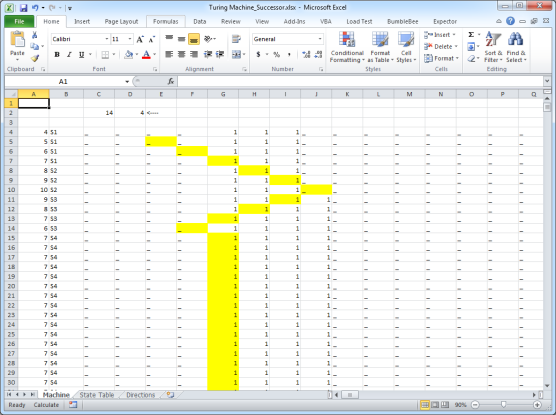
\includegraphics[width=\columnwidth]{fig/turing.png}
  \caption{A Turing machine implementation in Excel, using only formulas}
  \label{fig:visical}
  \end{center}
\end{figure} 

Secondly, spreadsheets are Turing complete, even without taking Visual Basic for Applications code into account. Using formulas only, you can construct a Turing machine, see Figure \ref{fig:visical}~\cite{Turing2013}. Without using formulas, it is not possible to update the tape on each move of the Turing machine. Moving the head is mimicked by using one row in the spreadsheet to represent one state of the tape. Each following line represents the state of the tape after one transition, and the head of the machine is visualized with conditional formatting.

\subsection{Maintainability issues are similar}

Finally spreadsheets suffer from typical software problems, including, but not limited to the issues below.

\textbf{Long life span} Sometimes, spreadsheets are created for one time use, and they are also thrown away after that use. More often they stay ‘alive’: enhanced with more data, reused for next year's budget or modified for a different department. Our research shows that spreadsheets have an average lifespan of five years~\cite{hermans_supporting_2011}.

\textbf{Many different users} During their lifespan, spreadsheets are frequently shared among coworkers. On average, twelve different people work with one spreadsheet during its life, performing a variety of tasks on them, including data entry, error checking and analysis~\cite{hermans_supporting_2011}.

\textbf{Lack of documentation} We found that only one in three spreadsheets contain documentation, and we are not even talking about technical documentation, but just something as basic as a manual on how to use the spreadsheet is lacking in two thirds of the spreadsheets we examined~\cite{hermans_supporting_2011}.

\textbf{Quality issues} Many accounts of big impact errors: From somewhat silly errors, like an overbooked Olympic stadium~\cite{Kelso2012}, to career wrecking data analysis mistakes~\cite{Herndon2014}, the stories of errors are numerous. The European Risk Interest Group keeps a list of these ‘spreadsheet horror stories’ on their website.\footnote{\url{www.eusprig.org/horror-stories}}

\section{Reflections on Spreadsheet Success factors}
Given the extreme wide adoption of spreadsheets, one could wonder why spreadsheets are as successful as they are. We believe there are a number of different reasons for their success.

\subsection{Live programming avant la lettre}

\begin{figure}
  \begin{center}
  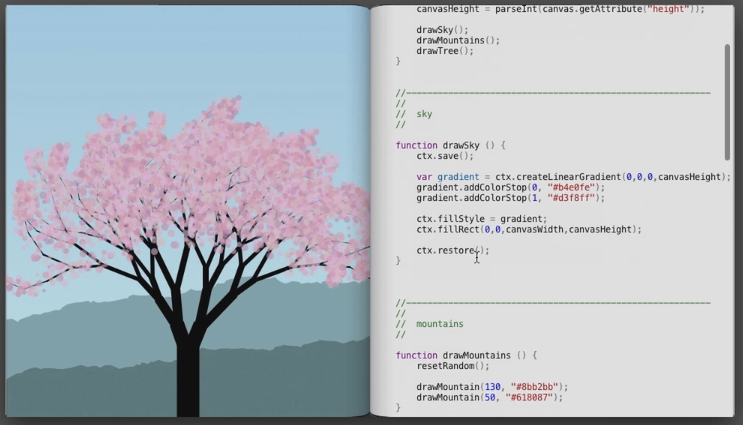
\includegraphics[width=\columnwidth]{fig/bret.png}
  \caption{Live programming: on the right the source code and on the left its instantiation of the code which changes immediately when the code is updated.}
  \label{fig:bret}
  \end{center}
\end{figure} 

Recently, ‘live programming’ has been made popular, among others by Bret Victor in his talk `Inventing on Principle'~\cite{Victor2012}. Figure \ref{fig:bret}, taken from Victor's talk, illustrates the idea of live programming: on the right, we have source code and on the left, we have the result of that code, in this case: a tree. Modifying the code will immediately affect the tree.
 
This idea however, often presented as a novelty in programming experiences, is exactly what happens when a user enters formulas in a spreadsheet. Immediately when the user presses enter on the keyboard, she sees the result. No compilation is needed. This liveness powers the flexibility of spreadsheets, often praised as their key success factor.

\subsection{Data, metadata and calculations in one view}
While researching spreadsheets, we have often asked the more tech savvy spreadsheet users why they did not use a more structured approach, like Microsoft Access \bas{If we are precise than Microsoft Access is a database, not a structured approach, the structured approach is not depending on the software, however using database software will force a structured approach while excel is not} . What we found was that the disconnect between the meta-data (designing the tables), the data (filling them) and the analysis (queries) was too hard for many users. The fact that all of those can be bundled in one view apparently makes it easier for non-programmers to keep an overview of what is going on. This is not that surprising, understanding dependencies of code is one of the challenges that developers still face, even advanced IDE's like Eclipse or Visual Studio do not solve this entirely. \todo{do we have a citation here?}

\subsection{One-click deployment}
Another problem that professional users face is the problem of deployment. Some more advanced users write, for example, Python scripts to analyze data. But how to get that to run on your neighbor's workstation, with a slightly different version of the operating system, a newer Office and different language settings? Spreadsheets are so universal that almost everyone has a spreadsheet program on their machine and the different programs can easily convert them. With that, a spreadsheet becomes an executable package with data and calculations packed together, that can run anywhere.

\section{Achievements} 
One of the approaches to \emph{end-user software engineering} research has been to transfer methods from software engineering to end-user languages, and this is an approach that has been applied eagerly in research into spreadsheets. This section presents an overview of successful approaches following this scheme.

\subsection{Testing}
One of the programming concepts that found its way to spreadsheets earliest is testing. 

\todo{summarize WYSIWYT}

The WYSIWYT framework was created~\cite{Rothermel1997} and subsequently validated~\cite{Rothermel2000} by Rothermel \emph{et al.}. Their evaluation showed that their approach had an average fault detection percentage of 81\% which is ``comparable to those achieved by analogous techniques for testing imperative programs." Other studies have confirmed the applicability of testing~\cite{Kruck2006}. The WYSIWYT methodology requires users to explicitly indicate what cells of a spreadsheet are correct and the system propagates the testedness of a cell to its dependents. Related is the elegant work of Burnett on spreadsheet assertions that uses a similar propagation system \cite{Burnett2003}.\todo{And indeed also Expector}

\subsection{Reverse Engineering} 
Like software, spreadsheets often suffer from a lack of documentation. In a field study, we found that only one in three spreadsheets have documentation~\cite{hermans_supporting_2011}. In the study we found this causes problems especially in situation where a spreadsheet is transferred: between colleagues, from a spreadsheet user to IT for migration or when a spreadsheet had to be reviewed by an auditor. In literature there have been a few approaches to extract knowledge from spreadsheets in order to assist understanding. 

\subsubsection{Extracting class diagrams}
There have been a number of approaches to extract class diagrams from spreadsheets. We ourselves have described a method to do so by observing that spreadsheets typically contain three things: data divided in groups, computations over these groups, and dependencies between them. This type of organization closely resembles that of object oriented systems, and thus groups of data were converted into classes, formulas into methods, and dependencies into associations~\cite{hermans_automatically_2010}. We implemented the extraction by creating a library of commonly used and well-defined spreadsheet patterns and implemented the. The implementation was evaluated on the EUSES corpus~\cite{fisher_euses_2005}. The patterns of the created library were found to be occurring in around 40\% of the corpus spreadsheets. For 50 randomly selected spreadsheets from the corpus, class diagrams were generated manually and compared with the output of the Gyro tool. In this set, 40\% of cases proved to be exact match and the rest had various degrees of mismatch with only 12\% having no relationship to the manual created benchmark.

Following this work, Cunha \emph{et al.}~\cite{cunha_automatically_2010} described an approach to infer ClassSheets models~\cite{engels_classsheets:_2005} from spreadsheets, by detecting and exploiting functional dependencies. Their method was validated in a method similar to ours. They manually extracted tables from 27 spreadsheet examples taken from \cite{management_2003}. They found that their method was able to detect correct ClassSheets in about 70\% of the cases.

Specifically focusing on the spreadsheets made by scientists, De Vos \emph{et al.}~\cite{vos_g.:_2012} have designed a methodology to extract ontologies in the form of class diagrams from spreadsheets. While their described method is currently manual, they state it could be automated too. 

%(maybe include) Isakowitz et al. proposed a related methodology to infer a logical layer of existing spreadsheets [10], but their process in not completely automatic, it requires human intervention in some cases.

\subsubsection{Dataflow visualization}
One could say that spreadsheets consist of two layers: \emph{visual}: the way in which cells are organized into rows, columns, data blocks and worksheets, and \emph{dependency}: the way in which cells refer to each other. The above approaches for extracting class diagrams have mainly focused on extracting information on the visual level. There have been a number of approaches that have worked on extracting and visualizing the underlying formula structure too, because it is often hard to understand how the formulas refer to each other, especially if this is not congruent with the way the formulas are laid out. 

We have studied this issue by performing a study at a large Dutch financial services company Robeco, to learn about the information needs that industrial spreadsheet users have when working with spreadsheets~\cite{hermans_supporting_2011}. The results confirmed that that most important information needs of spreadsheet users concern the structure of formula dependencies.

To meet this demand we developed an approach for automatic generation of leveled data-flow diagrams from spreadsheets. The diagrams can be used to visualize data in a spreadsheet and the dependencies between the data. 

Furthermore the diagrams can depict hierarchical structures like blocks of cells or different worksheets, as shown in Figure \ref{fig:worksheet-view}. We implemented the approach and evaluated it with a group of 27 users from Robeco, in the context of three transfer scenarios where spreadsheets were being transferred: between spreadsheet users, from users to auditors, and from users to IT engineers who were migrating spreadsheets to custom software applications. The results indicated that the professionals from Robeco consider the tool helpful; the visualizations help them to create story lines for explaining spreadsheets to colleagues, and they scale well to large and complex spreadsheets in use at Robeco. 

\begin{figure}
  \begin{center}
  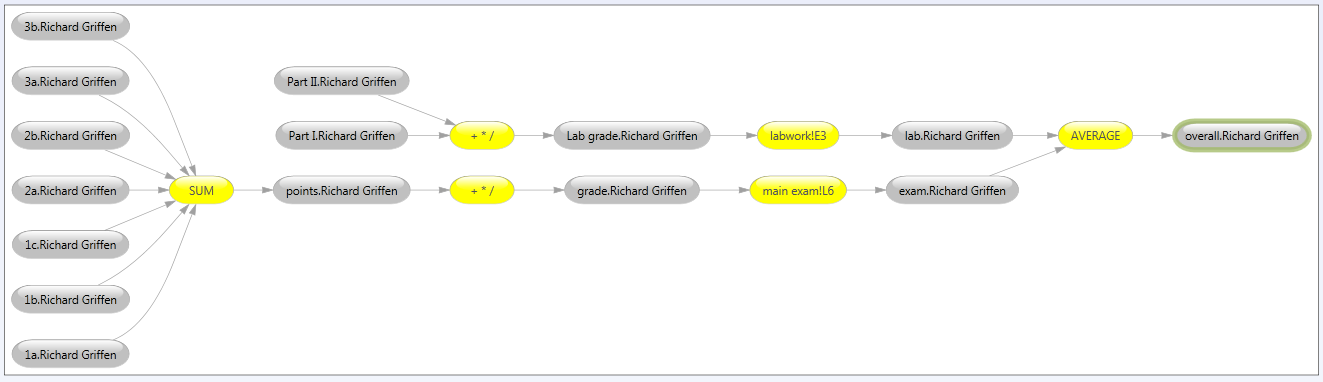
\includegraphics[width=\columnwidth]{fig/formula-view.png}
  \caption{Formula view of the Leveled Dataflow Visualization as presented in \cite{hermans_supporting_2011}}
  \label{fig:formula-view}
  \end{center}
\end{figure} 

\begin{figure}
  \begin{center}
  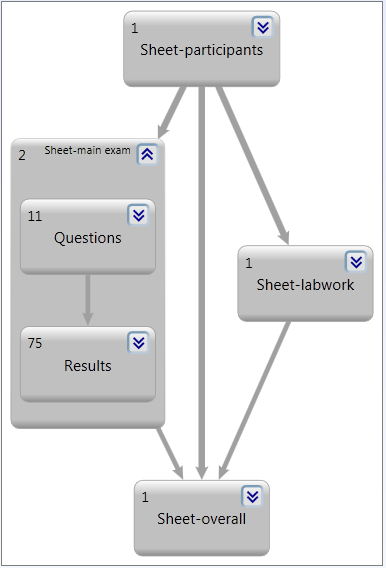
\includegraphics[width=5cm]{fig/worksheet-view.png}
  \caption{Worksheet view of the Leveled Dataflow Visualization as presented in \cite{hermans_supporting_2011}}
  \label{fig:worksheet-view}
  \end{center}
\end{figure} 

In addition to our work on dataflow visualization, there is also work specifically tailored towards the spreadsheets used by scientists~\cite{de_vos_methodology_2015}. In the paper De Vos \emph{et al.} propose a semi automatic method to infer the calculation workflow underlying a set of spreadsheets. The starting point of our methodology is, like in our approach, the cell dependency graph. The difference is that 1) De Vos \emph{et al.} automatically aggregate all cells in the graph that represent instances and duplicates of the same quantities, based on analysis of the formula syntax.

Furthermore the method needs an ontology of the spreadsheets domain as input, which is then used to prune the data flow graph by selecting only relevant nodes. In ~\cite{de_vos_methodology_2015} this is applied manually, however their goal is to integrate this into their algorithm in future work. They have performed three case studies showing that their generated calculation models
approximate the ground truth calculation workflows, both in terms of content and size, but are not a perfect match.

\subsection{Smell Detection} 
After focusing on extraction of documentation, we found out that spreadsheet users often prefer to work in spreadsheets over migrating them, hence we shifted our focus to helping users understand the complexity of spreadsheets and determine ways to improve them. For this, we took the idea of \emph{code smells} as inspiration, adapting it however, to be applicable to spreadsheets. 

\subsubsection{Formula-level Smell detection}
We started by defining smells on the formula level where we found that many smells defined for code also applied nicely to spreadsheets~\cite{hermans_detecting_2014}. As an example, consider conditional complexity. Most spreadsheet systems contain IF and other conditional formulas, so spreadsheet formulas too can suffer from conditional complexity, when many conditionals are nested within one formula.\todo{maybe add an example here}

Other code smells need small modifications to be applicable to spreadsheets: the \emph{many parameters} smell became \emph{many references}: a formula that references a long list of different ranges in a spreadsheet is as smelly as a method with lots of parameters, and the \emph{long method} smell became \emph{multiple operations}: a formula that uses a large number of different functions can be hard to understand.

After defining the smells for spreadsheets, we performed empirical evaluations to ascertain ourselves that the smells mattered to spreadsheet users. We first analyzed the occurrence of the smells with the EUSES corpus~\cite{fisher_euses_2005}, secondly, we conducted a series of case studies at Robeco, where we conducted ten case studies. 

\subsubsection{Spectrum-Based Smell Detection}
\todo{SBFL}

\subsubsection{Data Smell Detection}
Cunha \emph{et al.} studied smells in spreadsheets too, however they focus on smells in the data, such as cells that do not follow a normal distribution or have a big string distance to other cells in the same region, and thus might be typos. They analyzed 180 spreadsheets from the EUSES corpus, in which they found 3,841 cells suffering from their smells. By manual inspection of the cells, they confirmed that more than 20\% of the detected smelly cells point to a possible problem in the spreadsheet~\cite{cunha_towards_2012}.

Related work into smells in data was done by Barowy \emph{et al.} who present a tool called CheckCell that identifies cells that have an unusually high impact on the spreadsheet’s computations. In an evaluation, the authors showed that CheckCell outperforms standard outlier detection techniques. It successfully finds injected typographical errors produced by a generative model trained with data entry from 169,112 Mechanical Turk tasks~\cite{barowy_checkcell:_2014}.



In more recent work we have compared two datasets: one containing spreadsheets which users found unmaintainable, and a version of the same spreadsheets rebuilt by professional spreadsheet developers. The results show that the improved versions suffered from smells to a lesser degree, increasing our confidence that presence of smells indeed coincides with users finding spreadsheets hard to maintain~\cite{Jansen2015}.



\subsubsection{Structural Smell detection}
In addition to smells within a single worksheet of a spreadsheet, smells can occur in the way they are coupled also; just like with source code. We explored this phenomena too, leading to four `inter-worksheet smells': Inappropriate Intimacy, Feature Envy, Middle Man and Shotgun Surgery~\cite{hermans_detecting_2012-1}. We again performed a quantitative and qualitative evaluation of our approach. Firstly, we analyzed the EUSES~\cite{fisher_euses_2005} corpus, and investigated the occurrence of inter-worksheet smells. Secondly, we conducted a series of ten case studies at the above described company Robeco. In each study we analyzed a real-life spreadsheet, and discussed the located smells with the spreadsheet owner. \todo{Add results / conclusions / contributions of this study?} 

\subsection{Clone detection}
Like in source code, clones or `copy-pasting' occurs in spreadsheets too, although there are important differences. 
Copy-pasting in spreadsheets is common: spreadsheet users mimic abstraction by copying a similar formula down or left over multiple rows or columns. An example of this is given in the lower part of Figure {fig:ambig}, where the formulas in cells D2 and F2 are copied down and the formula in B2 is copied left.

\begin{figure}
  \begin{center}
  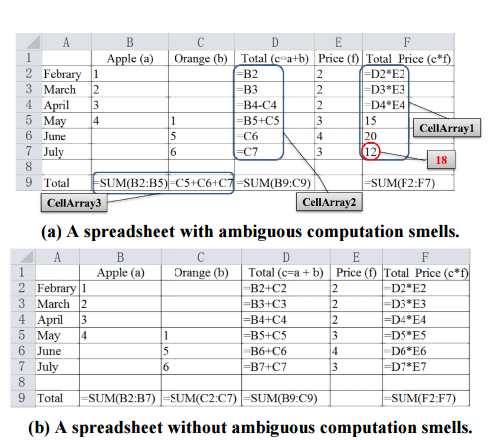
\includegraphics[width=\columnwidth]{fig/ambig.png}
  \caption{Two versions of a spreadsheet, with and without ambiguous computation. Taken from \todo{SC paper}}
  \label{fig:ambig}
  \end{center}
\end{figure} 

However, some forms of copying are error prone. In our research we have focused on \emph{data clones}: copies made with the `paste as values' option within Excel. We designed a detection algorithm~\cite{hermans_data_2013} to help spreadsheet users in finding and refactoring clones, based on existing clone detection algorithms working on source code~\cite{DBLP:conf/cascon/Johnson93}. In addition to exact clones, our approach also detects \emph{near-miss clones}, those where minor to extensive modifications have been made to the copied fragments~\cite{DBLP:conf/icsm/Roy09}. Our approach was  validated both quantitatively and qualitatively. Firstly, we analyzed the EUSES corpus~\cite{fisher_euses_2005} to calculate the precision and performance of our algorithm and to understand how often clones occur. Secondly, we performed two case studies: one with a large budget spreadsheet from our own university and a second one for a large Dutch non-profit organization, for which we analyzed 31 business critical spreadsheets.

\todo{maybe delete if we need space}Spreadsheets are not the only end-user artifacts that can suffer from cloning. There have been other efforts to apply clone detection outside of source code too. Alalfi \emph{et al.}~\cite{DBLP:conf/icsm/Alalfi2012} for example have successfully applied clone detection to Simulink models. For this purpose they adapted NiCad and were able to efficiently find exact, renamed and near-miss clones in Simulink models.

\subsection{Improving/re-engineering/Refactoring}
A final direction on which end-user research has focused on---a logical step after research on smells---is refactoring of end-users artifacts. 

%The first attempt to define refactorings for spreadsheets was made by O'Beirne, who took inspiration from both existing source code refactorings and his own experience in working with spreadsheets, he however did not evaluate his approach~\cite{obeirne_spreadsheet_2010}. 

Inspired by our work on spreadsheet smells, Badame and Digg~\cite{badame_refactoring_2012} developed a tool called RefBook that supported a number of refactorings for spreadsheet formulas including extract column, replace awkward formula, string to dropdown, introduce cell name, and extract literal. While some of their refactorings can relieve known code smells---for example extract column makes formulas shorter, thus addressing the \emph{multiple operations} smell---their refactorings were not directly related to smells. RefBook was evaluated on 28 users in an online experiment showing that RefBook increases spreadsheet programmer
productivity, increases the reliability of transformations, and increases the quality of spreadsheets. Furthermore they studied the EUSES corpus to show that their refactorings can be widely applied. For example, 27\% \todo{of spreadsheets?} contain some form of duplication, meaning that Extract Column could be applied to simplify the spreadsheet.

We subsequently defined refactorings corresponding to our smells~\cite{hermans_detecting_2014} and applied them to the 10 spreadsheets received from financial company Robeco, demonstrating that a combination of one or more refactorings from our set could relieve smells in 87\% of smelly formulas.

\subsection{Conclusion}
In conclusion, we conclude that a diverse range of approaches aimed at source code are applicable to end-user programming in general and spreadsheets in particular. From testing to smells, and from refactoring to reverse engineering, all transfers well and end-users benefit from it as much as professional developers do.

%This all has to do with understanding and improving quality we still want to support understanding domain/calculation.Our work and that of others was all 100\% automated, what we have learned, if we want to continue with reverse engineering, we need more support from the user, both the creator and human level intelligence (a generic user): we both want to do large studies with generic users like the labeling game and make support for users to add more (domain) knowledge to the sheets.

\section{Challenges} 
Now we have described the key success in the application of software engineering to spreadsheets, we direct our attention to challenges that still lie ahead of us. 

\subsection{End-user's perception and self perception}
One of the core challenges of performing research on end-user programming in general, is that users do not see themselves as programmers. In one case where we were working with an investment banker, who was even insulted when we, impressed with a risk management dashboard he built with Excel, called him a programmer. Because end-user programmers do not self-identify as developers, they often are unaware of tools, methods and techniques that could support them in their programming efforts.

The perception of end-user programmers as not being `real' programmers is not limited to how programmers view themselves, but also to how they are seen by others. Coworkers, especially those themselves trained as professional developers, often fail to recognize and sometimes even belittle their programming efforts, while professional developers in the workplace could offer great support and could ease our technology transfer issues. \bas{especially in the 'structured' translation of domain specific knowledge to technical implementation}

\subsection{Lack of Best Practices}
A challenge that follows the previous one is the lack of standards. As spreadsheets and their creators are not seen as source code and programmers respectively, they are often outside of the scope of a diverse range of professionalization efforts within companies. Software, but also numerous processes are standardized; spreadsheets on the other hand are rarely. While a number of spreadsheet standards exist\footnote{\url{http://www.fast-standard.org/}}\footnote{\url{http://www.ssrb.org/standards}}\footnote{\url{http://www.spreadsheetsafe.com/}}, these have to date not found widespread adoption, nor are any `lint tools' to check for spreadsheet compliance. 

The lack of standards means spreadsheets can be made in many different ways, this in turn inhibits easy comprehension and maintenance, but also makes it harder to automatically analyze and process spreadsheets.

\subsection{Lack of Data}
Spreadsheets often contain models and calculations of vital information to companies and therefore companies are often reluctant to share them with researchers. This is a big challenge with industrial research in general, and spreadsheets in specific. Contrary to source code, which developers often happily open source and share on online platforms like GitHub, spreadsheet users typically do not share their applications. While there are a number of public datasets available~\cite{fisher_euses_2005, Hermans2015, conf/msr/BarikLSSM15}, only one of these (\cite{Hermans2015}) stems from a company. And even then, we lack information about their creation and the maintenance process around them. Information that is often available for source code repositories, like issues, refactorings and version control history, are missing from spreadsheets, prohibiting us from deeply understanding the problems with spreadsheets. We have worked together with companies providing us with data~\cite{hermans_supporting_2011, hermans_detecting_2012, hermans_detecting_2012-1, hermans_detecting_2014, Jansen2015} enabling us to study spreadsheets \emph{in the wild}, however unfortunately, that came at the price of reduced repeatability, as we were not allowed to share these spreadsheets.

\subsection{Size of spreadsheets}

While many spreadsheets are relatively small, spreadsheets can also grow extremely large over their long lifespan. The biggest spreadsheet from the Enron set had no less than 175 worksheets, and about 10\% of spreadsheets in the corpus have 10 or more worksheets. Large spreadsheets, especially those with heavy connections between the worksheets are hard for users to understand and maintain. There have been several efforts to support spreadsheet users in comprehension. Igarashi \textit{et al.} developed a fluid visualization technique based on overlaid animation for better understanding of spreadsheets \cite{igarashi1998fluid}. However the animations were found to be radically degrading for spreadsheets larger than 400 cells. Compared to spreadsheets that are found in the industry, 400 cells is a very low limit. Shiozawa \textit{et al.} proposed a technique of cell dependence visualization in 3D based on an interactive lifting up operation \cite{shiozawa19993d}. Innovative in its approach, the prototype made use of OpenGL to implement the 3D graphics and was evidently resource consuming. However information regarding performance limits was not provided by the authors. Ballinger \textit{et al.} developed a visualization toolkit that could ease understanding of spreadsheets through visual abstractions in the form of images that emphasize on layout and dependency rather than values of cells \cite{ballinger2003spreadsheet}. The toolkit was successfully tested on a corpus of 259 spreadsheets but there was no information about the source or size of the spreadsheets. User-studies were not conducted and no details were given on whether users found it easy to understand the various types of images. Most notably, all of these projects have been abandoned and none of them found any industrial exposure.\todo{Sohon maybe you can add some work from your SEMS paper?DONE.} Thus it appears that although these tools typically perform well on laboratory examples, industrial adoption is far away for real-life spreadsheets, as 1) tools get unreasonably slow on large spreadsheets and 2) the abstractions in the visualization quickly lose their power for large spreadsheets with loads of dependencies. Fig.\ref{fig:ComplexDependence} shows the outcome of Excel's blue arrow based dependence tracing feature acting on a typical large and complex spreadsheet.

\begin{figure}
	\centering
	\setlength{\fboxsep}{0pt}
	\setlength{\fboxrule}{1pt}
	\fbox{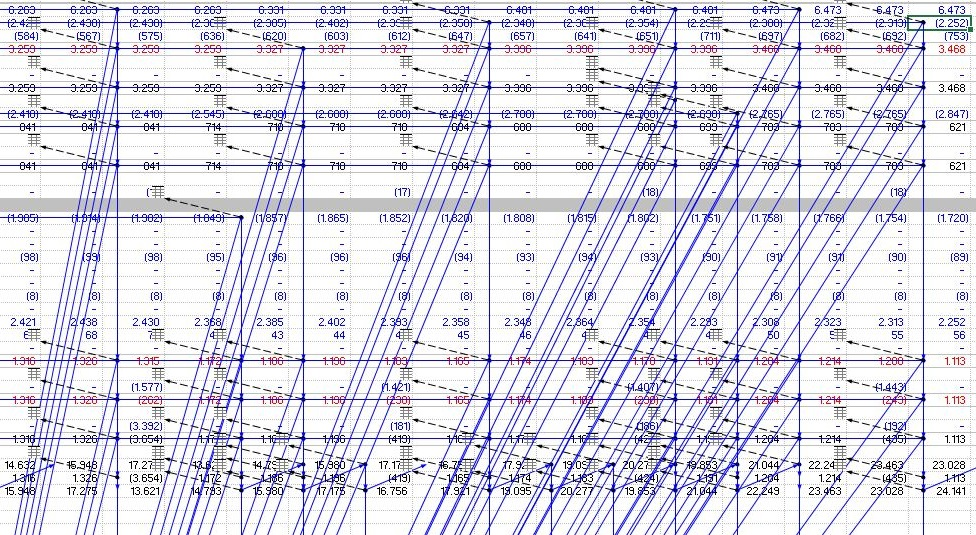
\includegraphics[width=\linewidth]{fig/ComplexDependence}}
	\caption{Complex Dependency Network in Spreadsheets}
	\label{fig:ComplexDependence}
\end{figure}

%For useful visualization we have to leave the cell level, want to look at the computation level (slicing)


\subsection{Technical issues} 
Finally, there are technical issues in processing spreadsheets and developing add-ins for a proprietary product like Microsoft Excel. 
Lack of open standards, and even when open, not very standardized (we have to reverse engineer stuff, link SCAM, also HPC/HEAT is not open, not willing to share)
Limited options for customization (undo/redo stack is not available, in the object model precedents do not go deeper than 1 level, objects model gets extended but not updated)

Obviously, one could steer away from these issues by implementing a system themselves (Forms/3 and Sestoft) or to build plugins for open source tools. Here however the tradeoff with realism is apparent too, building tools for Excel which is the number 1 spreadsheet solution increase the realism and impact of research tools.

\section{Future opportunities}
In the previous sections we have described a number directions in which the application of software engineering to spreadsheets  has proven to be successful. Testing, reverse engineering, smell detection, clone detection and refactoring have all been implemented and tested in practice to some extent. Given these achievements and the challenges we identified in terms of perception of end-users, best practices, lack of data, size and performance of spreadsheets, we identify the following viable directions for future work in the area of spreadsheet software engineering.

%\subsection{Continuation of the refactoring and testing work}
%In contrast to the work on smells that have been tried in practice and spurred numerous follow up works and has been picked up by a larger research community, refactorings and testing need to be made more applicable.

\subsection{Performance}
Understandability and maintainability are not the only issues with large spreadsheets, large spreadsheets can also suffer from serious performance problems. Some researchers have attempted to improve spreadsheet performance in various ways, for example, Pichitlamken \emph{et a.l}~\cite{7_pichitlamken_kajkamhaeng_uthayopas_kaewpuang_2010} proposed a method to offload a simulation model built in spreadsheets into a grid of computing resources, by splitting the problem in question into smaller problems that can be run in parallel independently. Their tool, while useful, was developed for a very specific set of conditions, making it difficult to generalize this line of work. A related effort is the work by Abramson et al. in \cite{6_abramson_roe_kotler_mather_2001} who presented ActiveSheets, a solution designed to evaluate ``otherwise sequential'' custom functions of Excel spreadsheets in the background, by creating a middle ware layer that gets the requests for evaluations. Once the evaluation request is received for a particular function it is immediately returns with a specific message to the spreadsheet, in order to allow the next function to start in parallel, if it is not dependent on this function's call. Meanwhile, the previous function's actual calculations are being processed in the background and possibly on multiple computational nodes, or a cluster. Finally, there is ExcelGrid \cite{10_nadiminti_chiu_teoh_luther_venugopal_buyya_2004}, in which a middle ware tool was designed and built connecting an Excel spreadsheet with either a private or a public cluster. For each type of clusters, a separate interface is developed to handle the communication of tasks. In their main experimental model, the user interactively provides the middle ware with the needed data and configuration to operate: input and output cells, and an executable file, which represents a specific software that will perform the actual computing operation on the data set provided. The partitioning here is simple: each cell represents a job, either on a vertical direction (row-based) or on a horizontal direction (column-based). ExcelGrid uses Excel spreadsheet as a tool for providing data to another software which needs the extensive computing resources. 

The fact that there is some preliminary research done in this direction, indicates that this is a problem worthy of more research. And, while the above tools and techniques do improve performance in the spreadsheets under study, they do not take the content of the spreadsheet into account, by for example identifying hotspots in the spreadsheets calculation. We believe that by combining HPC with smell detection and refactoring, tailored spreadsheet improvements could be made.

\subsection{Deeply understanding spreadsheets in the enterprise}
So far, work on spreadsheets, both ours and that of other research groups, have focused on individual spreadsheets and their users. In reality, spreadsheets are often part of a larger end-user ecosystem, where users, for example, import data from a datawarehouse, process it in a spreadsheet and then write a report about it in Word. We see the broadening of the scope of end-user programming as a very viable direction for future research. 

This research direction will aim to understand why people continue to resort to `home brew' solutions while there are software systems in place. What functionality or power do they miss in existing tools? Understanding what drives people to spreadsheets will support us in building supporting or replacing tools.

\subsection{Specializing on different types of spreadsheets}
Not all spreadsheets or other end-user artifacts are created equally. While working with spreadsheets in practice we have seen that there are several high-level classifications to be made. For example: many spreadsheets are used for time-series \todo{Bas, roep nog eens wat termen hier :-)}

\subsection{Support users in creating better spreadsheets}
In previous work we have tried to understand what causes spreadsheets to be error prone. Contrary to our initial hypotheses, studies have found that the level of complexity and coupling in spreadsheets is not that large \todo{ref F1F9 and Enron vs Euses}. So one could wonder what it is that makes spreadsheets error-prone and hard to understand. One hypothesis is that the interface of spreadsheets, with all its freedom for users in how to layout spreadsheets, is a double-edged sword. While allowing the users this total freedom, the interface is not supporting users in making the right choices. One solution we envision for the future is to help users to select the right formatting and also support them in changing the layout of the spreadsheet later in the process. 

\begin{figure}
  \begin{center}
  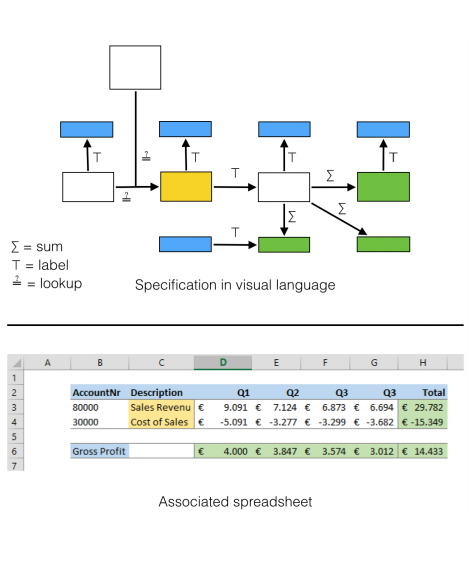
\includegraphics[width=\columnwidth]{fig/visualLanguage.png}
  \caption{We envision the visual language to look like this. On top there is the model the user would create and on the bottom we find the associated spreadsheet}
  \label{fig:visualLanguage}
  \end{center}
\end{figure} 


\subsection{Beyond formulas}
Spreadsheets themselves are changing, and many vendors, including Microsoft, are trying to enable spreadsheet developers to build more powerful programs. A few initiatives in this direction are ClickView, Tableau and PowerBI. Currently, these tools are certainly bringing more power to end-users, but are mainly concerned with helping them build new analyses and not with maintaining them. We envision end-users in this space making the same mistakes, and the creators of tools not focusing on end-user maintenance, maybe underestimating the longevity of the new artifacts created. We suspect that this new generation of end-user programming again will again suffer from end-user programming smells and be in need of testing and refactoring.

\section{Conclusion}
This paper presents an overview of research papers on applying methods from software engineering to spreadsheets. We first make the case that spreadsheets are code: they are used for similar problems, have similar expressive power and suffer for similar problems. We then reflect upon the success of spreadsheets, what makes them the world's most used programming languages for end-users? We assert their liveness, directness and easy deployment are core contributors to their widespread adoption. \todo{achieved research, challenges and future opportunities are missing}


\balance



% trigger a \newpage just before the given reference
% number - used to balance the columns on the last page
% adjust value as needed - may need to be readjusted if
% the document is modified later
%\IEEEtriggeratref{8}
% The "triggered" command can be changed if desired:
%\IEEEtriggercmd{\enlargethispage{-5in}}


\bibliographystyle{IEEEtran}
% argument is your BibTeX string definitions and bibliography database(s)
\bibliography{references}


% that's all folks
\end{document}


